\documentclass[runningheads]{llncs}

\usepackage[backend=biber]{biblatex}
\bibliography{AGI-book}

\usepackage[T1]{fontenc}
% T1 fonts will be used to generate the final print and online PDFs,
% so please use T1 fonts in your manuscript whenever possible.
% Other font encondings may result in incorrect characters.
%
\usepackage{graphicx}
% Used for displaying a sample figure. If possible, figure files should
% be included in EPS format.
%
% If you use the hyperref package, please uncomment the following two lines
% to display URLs in blue roman font according to Springer's eBook style:
%\usepackage{color}
%\renewcommand\UrlFont{\color{blue}\rmfamily}

\usepackage{amsmath}
\usepackage{amssymb}    % for \rightsquigarrow
\usepackage{wasysym}	% for frown face
\usepackage{mathrsfs} 	% for \mathscr
\usepackage{stmaryrd}
\usepackage{bm}
\usepackage{mathtools}		% to extend length of double harpoon arrows
\usepackage{tikz}
\usetikzlibrary{arrows,positioning,decorations.markings,shapes.multipart,shapes.geometric,shapes.arrows,tikzmark,calc}
\usepackage{tikz-cd}
\usepackage{sidecap}

\newcommand\logic[1]{{\color{gray}\mathsf{#1}}}

\makeatletter
\newcommand\mathcircled[1]{%
	\mathpalette\@mathcircled{#1}%
}
\newcommand\@mathcircled[3]{%
	\tikz[baseline=(math.base)] \node[draw,circle,inner sep=1pt] (math) {$\m@th#1#2$};%
}
\makeatother

\begin{document}
%
\title{Combining LLM and RL, and Logic Transformer}
%
%\titlerunning{Abbreviated paper title}
% If the paper title is too long for the running head, you can set
% an abbreviated paper title here
%
\author{King-Yin Yan \orcidID{0009-0007-8238-2442}}
%
\authorrunning{K-Y. Yan}
% First names are abbreviated in the running head.
% If there are more than two authors, 'et al.' is used.
%
\institute{\email{general.intelligence@gmail.com}}
%
\maketitle              % typeset the header of the contribution
%
\begin{abstract}
This paper has two main ideas:  The first is to explain two types of LLM (large language model) + RL (reinforcement learning) architectures, which are probably known on the internet but not explicitly stated.  The second idea is developed based on what we call ``Type L'' architectures.  Under this perspective, formal logic is essentially the same as natural language, and so LLMs (language models) are the same as logic processors.  Thus we introduce the Logic Transformer which may have advantages over traditional Transformers.

\keywords{AGI \and large language models \and reinforcement learning \and neural-symbolic integration}
\end{abstract}

\section*{Part I. \ LLM + RL architectures}

For ``string diagrams'' there are usually two conventions: 1) data are nodes, functions are edges: \tikz[baseline=(math.base)] \node[draw,circle,inner sep=1pt] (math) {$x$}; $\stackrel{f}{\longrightarrow}$ \tikz[baseline=(math.base)] \node[draw,circle,inner sep=1pt] (math) {$y$};  or alternatively 2) functions are nodes, data are edges: $\stackrel{x}{\longrightarrow}$ \tikz[baseline=(math.base)] \node[draw,circle,inner sep=1pt,fill=gray!20] (math) {$f$}; $\stackrel{y}{\longrightarrow}$.  In the following, I make explicit nodes for both functions (grey) and data (white), whereas edges merely represent linkages.

\begin{figure}
\label{fig:fundamental-forms}
\begin{tikzpicture}[every path/.style={thick},,decoration={
	markings,mark=at position 0.53 with {\arrow{>}}}]

\node[] (name) at (1.5,1.5) {\textbf{(RL)}};

\node[] (eye) at (-2, 0.25) {\includegraphics{eye-symbol.png}};
\node[] (mouth) at (-2, -0.25) {\includegraphics{mouth-symbol.png}};
\node[draw,thick,rectangle] (state) at (0, 0) {state $x$};
\node[draw,thick,circle,fill=gray!20] (RL) at (3.3, 0) {RL};
\node[draw,thick,cylinder,shape aspect=0.2,shape border rotate=90] (LTM) at (2.15,-0.1) {LTM};

\node[] (world) at (-1.3,1.3) {\includegraphics[scale=0.6]{world-symbol.png}};
\node[rotate=-40] (approx) at (-0.6,0.7) {\LARGE$\approx$};

\draw[postaction={decorate},rounded corners=12pt] (state.north) to ([yshift=18pt]state.north) to ([yshift=12pt]RL.north) to (RL.north);
\draw[postaction={decorate},rounded corners=12pt] (RL.south) to ([yshift=-12pt]RL.south) to ([yshift=-18pt]state.south) to (state.south);

\draw[-left to,shorten >= 5pt] (eye) -- (state.north west);
\draw[-left to,shorten <= 5pt] (state.south west) -- (mouth);
% \draw[double=gray!20,double distance=3pt,implies-{implies[fill=gray!20]}] (state.east) -- (LTM);
\node[draw, double arrow, double arrow head extend=1.5pt, fill=gray!20, minimum height=26pt, inner ysep=1.6pt] at (1.15,0) {};
\end{tikzpicture}
\qquad
\begin{tikzpicture}[node distance=-2pt,every path/.style={thick},every text node part/.style={align=center},decoration={
	markings,mark=at position 0.53 with {\arrow{>}}}]

\node[] (name) at (0,1.5) {\textbf{(Auto-encoder / LLM)}};

\node[] (world1) at (-2,0) {\includegraphics[scale=0.6]{world-symbol.png}};
\node[] (world2) at (2,0) {\includegraphics[scale=0.6]{world-gray.png}};

\node[rotate=90,rectangle,fill=white] (state) at (0, 0) {state $x$};
\draw[] (state.south east) -- (state.north east) (state.south west) -- (state.north west);

\node (compress1) [rotate=90, draw, trapezium, trapezium angle=-70, fill=gray!20, minimum height=28pt, inner xsep=3.9pt, above=0pt of state] {};
\node (compress2) [rotate=90, draw,trapezium, trapezium angle=70, fill=gray!20, minimum height=28pt, inner xsep=3.9pt, below=0pt of state] {};

\node[] (rho) at (0.1,0) {\large $\rho \qquad \quad \; \rho^{-1}$};
%\node[] (rho-1) at (1,0) {$\rho^{-1}$};

\end{tikzpicture}
\caption{The eye represents observations and the mouth (speech) actions.  Because RL has to maximize rewards, its internal representation (the state) must eventually approach a good approximation of the world.  LTM = long term memory, which works by associative recall and condensation, but will not concern us in this paper.  The auto-encoder, of which LLMs are a special case, works by compressing world-data (via $\rho$) and de-compressing (via $\rho^{-1}$) to re-construct the data (grey world).}
\end{figure}

First let's recall the \textbf{fundamental forms} of RL (Fig.\ref{fig:fundamental-forms} left) and auto-encoders (right).  The question is how to combine them, for which we can ignore the LTM module. Both RL and LLM have the ``state'' $x$ in common but there are subtle differences as to how to interpret these states (Fig.\ref{fig:types-AB}).  Initially my research favored \textbf{Type W}, where the LLM is interpreted as a \textbf{world model}.  This approach suffers the problem that we don't really understand the internal state (marked ``?'') of LLMs, which consists of many layers of Transformers and their intermediate token outputs, so we don't know how to ``merge'' the RL state with the LLM state.

% 反省的有效性,取决于: 这个 loop 如何训练,有效地训练。

% (Other researchers have proposed different taxonomies \cite{?}).
It seems that \textbf{Type L} would be easier to work with, and it is also the ``mainstream'' approach, of which RLHF seems to be an instance.  Here, the LLM simply loops over itself to form an RL loop.  The LLM models the ``spoken thoughts'' of human thinking, as found in text corpora.  These thoughts are interpreted as internal states of the RL.  Ever since Richard Montague's success in converting a fragment of English into formal logic \cite{Montague}, the line between formal logic and natural language is blurred.  We should not obsess with the idea that ``logic'' must be some kind of cryptic, undecipherable code.  This leads to a novel idea: \textit{the ``representation'' of human internal thought is just natural language.}  Type L also has the advantage that we can directly examine the internal state of an AGI.  What are currently called ``prompts'' is just \textbf{Working Memory}.

\begin{figure}
	\label{fig:types-AB}
\begin{tikzpicture}[node distance=-2pt,every path/.style={thick},decoration={
	markings,mark=at position 0.53 with {\arrow{>}}}]

\node[rectangle, align=left, text depth=5pt, anchor=west, text width=100pt] at (-1.5, 2.25) {\textbf{(Type L)} LLM as \\ language model};

\node[draw,thick,dashed,rectangle, minimum height=66pt, rounded corners=10pt, minimum width=50pt, label=right:RL] (RL) at (2, 0) {};
\node (state) [draw,rectangle split,rectangle split parts=2,minimum width=3em] at (0, 0) {$x_{t}$ \nodepart{two} $x_{t+1}$};

\node[] (eye) at (-1.5, 0.27) {\includegraphics{eye-symbol.png}};
\node[] (mouth) at (-1.5, -0.27) {\includegraphics{mouth-symbol.png}};

\node[] (speech1) at (2,1.8) {\includegraphics[scale=0.5]{speech-symbol.png}};
\node[] (speech2) at (2,-1.8) {\includegraphics[scale=0.5]{speech-gray.png}};

\node (compress1) [draw,trapezium,trapezium angle=-70, fill=gray!20, minimum height=25pt, inner xsep=-6.5pt, anchor=south] at (2,0) {\footnotesize NL${}^{-1}$};
\node (compress2) [draw,trapezium,trapezium angle=70, fill=gray!20, minimum height=25pt, inner xsep=-2pt, below=0pt of compress1] {\footnotesize NL};

% \node (stateA) [rectangle,minimum width=35pt, minimum height=5pt, above=0pt of compress1] {};
% \draw(stateA.south west) -- (stateA.north west) -- (stateA.north east) -- (stateA.south east);
% \node (stateB) [rectangle,minimum width=35pt, minimum height=5pt, below=0pt of compress2] {};
% \draw(stateB.north west) -- (stateB.south west) -- (stateB.south east) -- (stateB.north east);

% \draw[dashed] (stateA.east) to ([yshift=-5pt]state.north west);
% \draw[dashed] (stateB.east) to ([yshift=5pt]state.south west);

\draw[-left to, shorten >= 3pt] (eye) -- ([yshift=7pt]state.west);
\draw[-left to, shorten <= 3pt] ([yshift=-7pt]state.west) -- (mouth);

\draw[postaction={decorate},rounded corners=12pt] (state.north) to ([yshift=27pt]state.north) to ([yshift=14pt]compress1.north) to (compress1.north);
\draw[postaction={decorate},rounded corners=12pt] (compress2.south) to ([yshift=-14pt]compress2.south) to ([yshift=-27pt]state.south) to (state.south);
\end{tikzpicture}
\qquad \quad
\begin{tikzpicture}[node distance=-2pt,every path/.style={thick},decoration={
	markings,mark=at position 0.53 with {\arrow{>}}}]

\node[align=left, anchor=west, text width=100pt] at (-1, 2) {\textbf{(Type W)} LLM as \\ world model};

\node[draw,thick,circle,fill=gray!20] (RL) at (1.5, 0) {RL};
\node (state) [draw,rectangle split,rectangle split parts=2,minimum width=3em] at (0, 0) {$x_{t}$ \nodepart{two} $x_{t+1}$};

\node[] (world1) at (-2,1.7) {\includegraphics[scale=0.5]{world-symbol.png}};
\node[] (world2) at (-2,-1.7) {\includegraphics[scale=0.5]{world-gray.png}};

\node (compress1) [draw,trapezium,trapezium angle=-70, fill=gray!20, minimum height=35pt, inner xsep=1pt, anchor=south] at (-2,0) {};
\node (compress2) [draw,trapezium,trapezium angle=70, fill=gray!20, minimum height=35pt, inner xsep=1pt, below=of compress1] {};

\node (stateA) [draw,trapezium,trapezium angle=-70, fill=white, minimum height=6pt, inner xsep=4pt, above=-22pt of compress1] {?};
\node (stateB) [draw,trapezium,trapezium angle=70, fill=white, minimum height=6pt, inner xsep=4pt, below=-22pt of compress2] {?};

\draw[dashed] (stateA.east) to [edge label=?] ([yshift=-5pt]state.north west);
\draw[dashed] (stateB.east) to [edge label'=?] ([yshift=5pt]state.south west);

\draw[postaction={decorate},rounded corners=12pt] (state.north) to ([yshift=14pt]state.north) to ([yshift=15pt]RL.north) to (RL.north);
\draw[postaction={decorate},rounded corners=12pt] (RL.south) to ([yshift=-15pt]RL.south) to ([yshift=-14pt]state.south) to (state.south);
\end{tikzpicture}
\caption{Two types of RL + LLM architectures. NL${}^{-1}$ is a map that compresses natural language to a hidden representation (not shown explicitly).}
\end{figure}

\section*{Part II. \ Logic Transformer}

\begin{SCfigure}[50]
	\label{fig:she-loves-him}
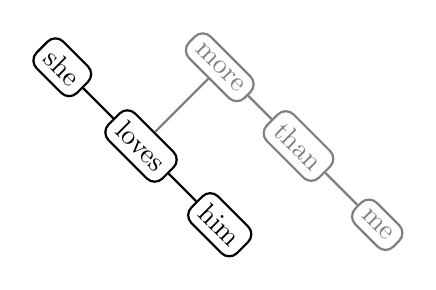
\begin{tikzpicture}[every path/.style={thick}]

\node (she) [draw,rectangle,rounded corners=4pt,rotate=-45] at (-1, 1) {she};
\node (loves) [draw,rectangle,rounded corners=4pt,rotate=-45] at (0, 0) {loves};
\node (him) [draw,rectangle,rounded corners=4pt,rotate=-45] at (1, -1) {him};
\node (more) [draw,gray,rectangle,rounded corners=4pt,rotate=-45] at (1, 1) {more};
\node (than) [draw,gray,rectangle,rounded corners=4pt,rotate=-45] at (2, 0) {than};
\node (me) [draw,gray,rectangle,rounded corners=4pt,rotate=-45] at (3, -1) {me};

\draw[] (she) -- (loves) -- (him);
\draw[gray] (loves) -- (more) -- (than) -- (me);

\end{tikzpicture}
\caption{Example of a linguistic tree (a connected graph without loops or double edges).  From a Chomskyan perspective, any NL sentence can fit into a tree structure.  This example starts with a simple relation, she-loves-him, and the ``love'' node is modified by a ``more'' clause.  Let's not dwell too deep into the details of this example, as machine-learning will fill in such details.}
\end{SCfigure}

As we know, LLMs predicts the next word per each iteration.  The number of possible natural-language sentences is an astronomical figure (if not $\infty$), so it is infeasible on any real computer to represent probability distributions over this set.  However, as vocabulary size is finite, the conditional probabilities $\mathbb{P}$(next word | prior words, context) is manageable.  This is part of what makes LLMs so efficient -- by decomposing sentences into words.

For a long time I tried to analyze the Transformer (Self Attention) from a symbolic-logic point of view, but could not interpret the meaning of \textbf{tokens} -- whether they should correspond to logic propositions, or sub-propositional symbols?  The question is how to reconcile these two views:
\begin{equation}
\nonumber
\hspace{-1cm} 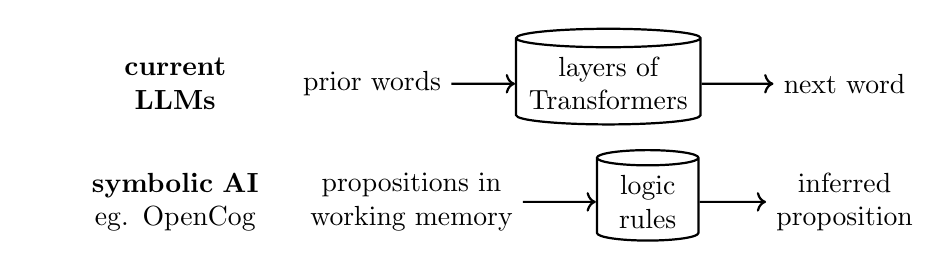
\begin{tikzpicture}[align=center, every path/.style={thick}]
\node[text width=100pt] at (-5.5, 0) {\textbf{current\\LLMs}};

\node (inputs1) [] at (-3,0) {prior words};
\node (KB1) [draw,thick,cylinder,shape aspect=0.1,shape border rotate=90,text width=60pt] at (0,0) {layers of\\Transformers};
\node (outputs1) [] at (3,0) {next word};

\draw[->] (inputs1) edge (KB1) (KB1) -- (outputs1);

% -------------------------------

\node[text width=100pt] at (-5.5, -1.5) {\textbf{symbolic AI}\\eg. OpenCog};

\node (inputs2) [] at (-2.5,-1.5) {propositions in\\working memory};
\node (KB2) [draw,thick,cylinder,shape aspect=0.15,shape border rotate=90,text width=30pt] at (0.5,-1.5) {logic\\rules};
\node (outputs2) [] at (3,-1.5) {inferred\\proposition};

\draw[->] (inputs2) edge (KB2) (KB2) -- (outputs2);
\end{tikzpicture}
\end{equation}
Finally I had a break-through insight that a symbolic-logic Transformer should output \textbf{atomic propositions} that modifies only one part of a linguistic tree at a time (Fig.\ref{fig:she-loves-him}).


Having convinced ourselves that LLMs can be a model of \textit{internal} thoughts, we wonder if the Transformer can be re-formulated as some kind of logic engine or general \textbf{rewriting system}, defined by rewriting \textbf{rules} that can be learned via gradient descent?

In order for such rules to be \textbf{differentiable}, we can't have $N$ rules at one moment and then suddenly $N+1$ rules the next moment (that would not be differentiable).  The only solution I can think of is to maintain a \textit{fixed} number, $M$, of rules.  Every rule may potentially ``morph'' into any other rule in this space of rules.  The set of rules would look like a \textit{rectangular} matrix:

\begin{equation}
\begin{aligned}
\mbox{rule 1:} & \quad \boxed{X^1_{11}... X^1_{1I}} \;\wedge\; \boxed{X^1_{21} ... X^1_{2I}} \;\wedge\;...\; \boxed{X^1_{K1} ... X^1_{KI}} \rightarrow \boxed{X^1_{01} ... X^1_{0I}} \\
\mbox{rule 2:} & \quad \boxed{X^2_{11}... X^2_{1I}} \;\wedge\; \boxed{X^2_{21} ... X^2_{2I}} \;\wedge\;...\; \boxed{X^2_{K1} ... X^2_{KI}} \rightarrow \boxed{X^2_{01} ... X^2_{0I}} \\
.... & \quad .... \\
\mbox{rule M:} & \quad \boxed{X^M_{11}... X^M_{1I}} \;\wedge\; \boxed{X^M_{21} ... X^M_{2I}} \;\wedge\;...\; \boxed{X^M_{K1} ... X^M_{KI}} \rightarrow \boxed{X^M_{01} ... X^M_{0I}}
\end{aligned}
\end{equation}

For a rule to be applicable, its atoms must match with propositions in Working Memory.  An atom may contain constants (such as ``Socrates'', that must be matched correspondingly) or variables (such as $x$, that matches any entity).  To achieve this, I introduce a trick called \textbf{cylindrification factor} (Fig.\ref{fig:cylindrify-example}).

\begin{figure}
	\includegraphics[scale=.6]{cylindrify-example.png}
	\caption{Illustration of the cylindrification factor $\gamma$.}
	\label{fig:cylindrify-example}
\end{figure}

To make \textbf{variable substitution} differentiable is even trickier.  Consider this logic rule:
\begin{equation}
\logic{father}(X_1,X_2) \wedge \logic{father}(X_2,X_3) \rightarrow \logic{grand\hbox{-}father}(X_1,X_3)
\end{equation}
We have to imagine some ``slots'' where we ``select'' variables using weights and \textbf{softmax}:
\vspace{-0.2cm} \begin{equation}
\logic{father}(
\begin{tikzpicture} \draw[line width=3pt, gray!50] (0.2,0.9) -- (0.2,0) (0.5,0.9) -- (0.5,0) (0.8,0.2) -- (0.8,0); \draw[thick] (0,0) to (1,0); \end{tikzpicture})
\wedge
\logic{father}(
\begin{tikzpicture} \draw[line width=3pt, gray!50] (0.2,0.2) -- (0.2,0) (0.5,0.9) -- (0.5,0) (0.8,0.9) -- (0.8,0); \draw[thick] (0,0) to (1,0); \end{tikzpicture})
\rightarrow
\logic{grand\hbox{-}father}(
\begin{tikzpicture} \draw[line width=3pt, gray!50] (0.2,0.9) -- (0.2,0) (0.5,0.2) -- (0.5,0) (0.8,0.9) -- (0.8,0); \draw[thick] (0,0) to (1,0); \end{tikzpicture})
\end{equation}
The actual implementation leads to formulas like these:
\begin{align}
\nonumber
& \qquad \qquad \tikzmark{Y1}
\setlength{\fboxrule}{3pt}
\fcolorbox{gray!50}{white}{$\hat{x}^1$}
\qquad
\tikzmark{Y2} \fcolorbox{gray!50}{white}{$\hat{x}^2$}
\qquad
\tikzmark{Y3} \fcolorbox{gray!50}{white}{$\hat{x}^3$} \\
& \qquad w_{ij}^k \\
& \nonumber \\
& \logic{father}(\tikzmark{X11} x_{11}, \tikzmark{X12} x_{12}, \tikzmark{X13} \bullet_{13}) \wedge
\logic{father}(\tikzmark{X21} \bullet_{21}, \tikzmark{X22} x_{22}, \tikzmark{X23} x_{23}) \rightarrow \logic{grand\hbox{-}father}(x_1,\bullet_2,x_3)
\nonumber

\begin{tikzpicture}[remember picture,overlay]
\draw (pic cs:Y1) +(10pt,-7pt) -- ($ (pic cs:X11) +(7pt,12pt) $);
\draw (pic cs:Y1) +(10pt,-7pt) -- ($ (pic cs:X12) +(7pt,12pt) $);
\draw (pic cs:Y1) +(10pt,-7pt) -- ($ (pic cs:X13) +(7pt,12pt) $);
\draw (pic cs:Y1) +(10pt,-7pt) -- ($ (pic cs:X21) +(7pt,12pt) $);
\draw (pic cs:Y1) +(10pt,-7pt) -- ($ (pic cs:X22) +(7pt,12pt) $);
\draw (pic cs:Y1) +(10pt,-7pt) -- ($ (pic cs:X23) +(7pt,12pt) $);
\draw (pic cs:Y2) +(10pt,-7pt) -- ($ (pic cs:X11) +(7pt,12pt) $);
\draw (pic cs:Y2) +(10pt,-7pt) -- ($ (pic cs:X12) +(7pt,12pt) $);
\draw (pic cs:Y2) +(10pt,-7pt) -- ($ (pic cs:X13) +(7pt,12pt) $);
\draw (pic cs:Y2) +(10pt,-7pt) -- ($ (pic cs:X21) +(7pt,12pt) $);
\draw (pic cs:Y2) +(10pt,-7pt) -- ($ (pic cs:X22) +(7pt,12pt) $);
\draw (pic cs:Y2) +(10pt,-7pt) -- ($ (pic cs:X23) +(7pt,12pt) $);
\draw (pic cs:Y3) +(10pt,-7pt) -- ($ (pic cs:X11) +(7pt,12pt) $);
\draw (pic cs:Y3) +(10pt,-7pt) -- ($ (pic cs:X12) +(7pt,12pt) $);
\draw (pic cs:Y3) +(10pt,-7pt) -- ($ (pic cs:X13) +(7pt,12pt) $);
\draw (pic cs:Y3) +(10pt,-7pt) -- ($ (pic cs:X21) +(7pt,12pt) $);
\draw (pic cs:Y3) +(10pt,-7pt) -- ($ (pic cs:X22) +(7pt,12pt) $);
\draw (pic cs:Y3) +(10pt,-7pt) -- ($ (pic cs:X23) +(7pt,12pt) $);
\end{tikzpicture}
\end{align}
\begin{equation}
\hat{x}^k \mathrel{:}= \underset{\text{predicates}}{\forall i \in} \; \underset{\text{arguments}}{\forall j \in} \left\langle \mathrm{soft}\max_{ij} w_{ij}^k \; , \; x_{ij} \right\rangle
\end{equation}
which is similar to the \textbf{Self-Attention} of Transformers:
\begin{equation}
\text{Attention}(\mathbf{Q,K,V}) = \text{soft}\max  \frac{\langle \mathbf{Q,K} \rangle}{\sqrt{d_k}} \mathbf{V}
\end{equation}
except that softmax does not commute with inner products, so they are not exactly equivalent, but qualitatively similar.  Let's pause for a moment to reflect that we tried to substitute variables (some kind of syntactic manipulation), and ended up with something like Self-Attention.  Also recall that Self-Attention originated as a kind of \textbf{content-addressable memory} for Neural Turing Machines, invented for its differentiability.

A final obstacle concerns the limitations of first-order logic.  As Ben Goertzel pointed out during an online discussion, my earlier design lacked mechanisms for handling \textbf{Skolem functions} and thus existential quantifiers.  One way to get around this problem is to define $\exists$ via a set of \textbf{higher-order logic} rules.  Without explicitly specifying how to do so (though I believe this can be done), we simply use a more powerful ``higher-order'' logic in the sense that rules admit substitutions in all (predicate or argument) positions, and hope that machine learning will learn the required axioms.

Armed with these ideas, it is not too difficult to work out a new kind of differentiable ``Logic Transformer'' (Fig.\ref{fig:string-diagram}).  A detailed explanation is contained in my on-going research thesis \cite{}.

\begin{figure}
	\hspace{-3cm}
	\includegraphics[scale=.7]{logic-Transformer-string-diagram-3.png}
	\caption{String diagram of the Logic Transformer.  The {\LARGE\color{gray}\RIGHTarrow} indicates \textbf{internal data} supplied by the Transformer, similar to the Q,K,V matrices in traditional Transformers.  These are modified through ``learning'' or training.  The 2 \RIGHTarrow's \ are \textbf{inputs} to the Transformer, this is matched with the 2 \textbf{outputs} on the right of the diagram.  Tags {\color{gray}$[M,N,...]$} indicate the \textbf{dimensions} of data streams.}
	\label{fig:string-diagram}
\end{figure}

\section*{Conclusions}

The significance of combining RL and LLM is such that the system can \textit{think in loops}, eliminating thoughts that contradict accepted truths, thus achieving genuine, logically coherent understanding, instead of just parroting human speeches.  This would also solve the problem of ``hallucinations''.  The remaining question is how to train the Type L model \textit{efficiently}, but this is more of an engineering rather than theoretical problem.

A very interesting question concerning Part II is how to handle \textbf{variable-length propositions}?  If this could be done, the neural network may have a form very close to or even identical to current Transformers...

%
% ---- Bibliography ----
%
% BibTeX users should specify bibliography style 'splncs04'.
% References will then be sorted and formatted in the correct style.
%
% \bibliographystyle{splncs04}
\printbibliography

\end{document}
